\documentclass[french]{article}
\usepackage[T1]{fontenc}
\usepackage[utf8]{inputenc}
\usepackage{lmodern}
\usepackage[a4paper, margin=2.5cm]{geometry}
\usepackage{babel}
\usepackage{amsmath}
\usepackage{amsfonts}
\usepackage{amssymb}
\usepackage[dvipsnames]{xcolor}
\usepackage{wrapfig}
\usepackage{graphicx}


\author{Badr YOUBI IDRISSI}
\title{\'Evolution de la quantité de travail d'un centralien}
\begin{document}
\maketitle
\section{Introduction et Modélisation}

    \begin{wrapfigure}{r}{0.25\textwidth}
        \begin{center}
            \includegraphics[width=0.23\textwidth]{Figures/Eisenhower.png}
        \end{center}
    \end{wrapfigure}
    La vie à Centrale peut être très chargée! pour s'armer contre l'interminable 
    flux de travail, il existe un outil d'organisation fort utile.
    La matrice d'Eisenhower est une grille à 4 cases qui classifie les tâches. Ce qui 
    aide à se fixer des priorités. Le but de ce modèle est d'étudier
    l'évolution du travail restant en fonction du temps, de son urgence et de son importance.
    
    Pour pouvoir utiliser des EDP je me place dans un cadre continu : $\Omega$ est
     l'espace (urgence, importance). Une tâche est représenté par 
    une gaussienne de moyenne $(\mu_x,\mu_y)$.
    Ceci peut être justifié en décrivant un travail donné comme plusieurs composantes
     d'importance et d'urgence variant
    autour de la moyenne. L'écart type $\sigma$ de représente l'étalement de cette décomposition.

    \subsection{\'Equation}
    Soit $\Omega = [0,1]^2$,
    
    \begin{equation}\label{EDP}
        \frac{\partial u}{\partial t} + \lambda\frac{\partial u}{\partial x} + \nu.u = \rho 
    \end{equation}
    \begin{alignat*}{6}
        u \;:\; &\text{\;Densité de travail restant} \\
        \lambda \;:\; &\text{\;Vitesse de l'augmentation en urgence}\\
        \nu \;:\; &
        \text{\;Efficacité} = \frac{1}{\tau(x,y)} \text{ avec } \tau(x,y) 
        \text{ le temps caractéristique de complétion d'une tâche en} \,(x,y)
    \end{alignat*}

    \subsection{Explications et précisions}
    On réecrit l'équation ansi : $\frac{\partial u}{\partial t} = \rho - \nu.u - \lambda\frac{\partial u}{\partial x}$. 
    Le terme $\rho$ est la source de travail (Ex: "Mini" projet d'EDP). Puis $ - \lambda\frac{\partial u}{\partial x}$ 
    correspond au transport en urgence : le plus le temps passe le plus chaque tâche devient plus urgente 
    (cf. Date de rédaction ci-dessus). Ensuite $\nu.u$ est le travail fourni par un centralien aléatoire. Pour $(x,y)$ fixé, le travail fourni 
    est logiquement proportionnel au travail restant. Il reste à determiner la dépendance en urgence et en importance 
    de l'éfficacité du centralien. Dans ce modèle on pose :
    \begin{align}
        \forall(x,y)\in\Omega, \; \lambda(x,y) &= C(1+y)^2 \\
        \forall(x,y)\in\Omega, \; \nu(x,y) &= (L_4-L_1)x+(L_2-L_1)y+(L_1+L_3-L_4-L_2)xy+L_1
    \end{align}
    

    \begin{wrapfigure}{r}{0.30\textwidth}
        \begin{center}
            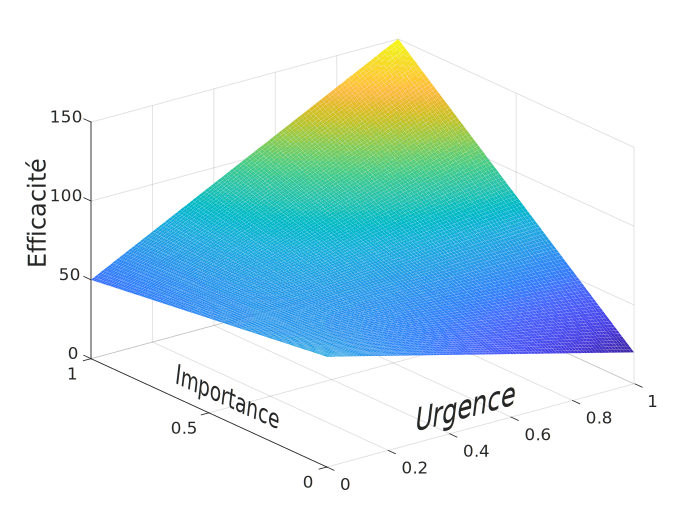
\includegraphics[width=0.30\textwidth]{Figures/Efficacite.png}
        \end{center}
        \vspace{-40pt}
    \end{wrapfigure}

        Avec $C > 0$ une constante de "convection". La fonction $\lambda$ reflète le fait 
        que les taches importantes sont de manière générale deviennent plus urgentes que celles qui le sont moins.
    Et $L_i > 0$ les valeurs de l'efficacité en $\{(0,0),(1,0),(1,1),(1,0)\}$. la fonction 
    $\nu$ ne fait qu'interpoler continuement entre ces valeurs. Les valeurs $L_i$ 
    caractérisent la personne qui accomplit les taches. Par exemple un grand $L_1$ 
    relativement aux autres signifie que  la personne a une tendance à effectuer des 
    taches non urgentes et non importantes. (Procrastination!)
    
    
    \section{Simulation}
    \subsection{Formulation variationnelle et résolution numérique}
    L'équation ci dessus est hyperbolique si l'on prends en compte que les dimensions "spatiales".
    Ceci fait que la résolution théorique introduit dans le cours n'est plus la même. J'ai essayé d'appliquer la méthode
    variationnelle directement mais sans succès (La résolution numérique finissait toujours par diverger). J'ai donc enlevé le terme problèmatique
    de 'convection' et je l'applique dans la boucle de résolution plutot que dans la formulation variationnelle. On fait en plus de ceci l'approximation 
    $\frac{\partial u^{(m)}}{\partial t} \approx \frac{u^{(m)} - u^{(m-1)}}{\delta t}$ On a donc l'équation
    \begin{alignat*}{10}
        \frac{u^{(m)} - u^{(m-1)}}{\delta t} + 
        \textcolor{Red}{\left( \lambda\frac{\partial u}{\partial x}\right)} 
        + \nu.u^{(m)} &= \rho^{(m)} \\
        \forall v \in \mathcal{D}(\Omega) \; \frac{1}{\delta t} \int_{\Omega} u^{(m)}v - u^{(m-1)}v + \int_{\Omega} \nu.u^{(m)}v
        &= \int_{\Omega} \rho v
    \end{alignat*}
    On calcul donc itérativement $u$. Pour prendre en compte le terme convectif, dans cette même boucle de résolution, on applique la fonction convect de freefem 
    \subsection{Résultats et Analyse}
    Total travail important non fait (Low Produc) 3607.78
    Total travail important non fait (High Produc)2058.24
    \subsection{Conclusion}
    
\end{document}
